\documentclass[11pt]{article}
\usepackage[T1]{fontenc}
\usepackage{lmodern}
\usepackage[margin=1in]{geometry}
\usepackage{amsmath,amssymb,amsthm,mathtools}
\usepackage{booktabs,array,longtable}
\usepackage{xcolor,microtype,fancyhdr,enumitem,tikz}
\usepackage[hyphens]{url}
\usepackage{xurl}
\usepackage[hypertexnames=false,colorlinks=true,linkcolor=blue!45!black,
 citecolor=blue!45!black,urlcolor=blue!45!black]{hyperref}
\usepackage{listings}
\setlist{itemsep=3pt,topsep=5pt}
\lstset{basicstyle=\ttfamily\footnotesize,breaklines=true,
 columns=fullflexible,keepspaces=true,frame=single,rulecolor=\color{black!15}}
\pagestyle{fancy}\fancyhf{}
\fancyhead[L]{\small Taylor and Cauchy in iPRA}
\fancyhead[R]{\small Finite quantitative proofs}
\fancyfoot[C]{\thepage}
\setlength{\headheight}{14pt}
\setlength{\emergencystretch}{2em}
\newtheorem{theorem}{Theorem}[section]
\newtheorem{lemma}[theorem]{Lemma}
\newtheorem{proposition}[theorem]{Proposition}
\newtheorem{corollary}[theorem]{Corollary}
\theoremstyle{definition}
\newtheorem{definition}[theorem]{Definition}
\newtheorem{remark}[theorem]{Remark}
\newcommand{\N}{\mathbb N}
\newcommand{\Z}{\mathbb Z}
\newcommand{\Q}{\mathbb Q}
\newcommand{\C}{\mathbb C}
\newcommand{\R}{\mathbb R}
\newcommand{\ipra}{\mathsf{iPRA}}
\newcommand{\PR}{\mathsf{PR}}
\newcommand{\abs}[1]{\left|#1\right|}
\newcommand{\norm}[1]{\left\lVert#1\right\rVert_1}
\newcommand{\dd}{\,\mathrm d}
\newcommand{\code}[1]{\texttt{#1}}
\newcommand{\clD}{\overline D}
\newcommand{\Trap}{\mathcal T}
\newcommand{\Int}{\mathcal I}
\title{Taylor's theorem and Cauchy's integral formula\\
in intuitionistic primitive recursive arithmetic}
\author{A constructive proof package prepared for Vladimir Reshetnikov}
\date{November 15, 2026}
\hypersetup{pdftitle={Taylor's theorem and Cauchy's integral formula in iPRA},
 pdfauthor={Prepared for Vladimir Reshetnikov},
 pdfsubject={Complete quantitative human proofs and an explicit Lean formalization plan}}

\begin{document}
\maketitle
\begin{abstract}
We prove constructive versions of Taylor's theorem with integral remainder,
its factorial error bound and its Peano form, and Cauchy's integral formula
on a circle. We also derive all higher Cauchy derivative formulas and a
complex Taylor expansion with a primitive recursive convergence rate.
Input functions have fixed primitive recursive rational approximation
procedures, bounds and uniform regularity certificates. These are explicit
arithmetical hypotheses; they are not extracted from qualitative
differentiability by an implicit compactness principle.

Two finite certificates carry the proofs. A single weighted derivative jet
gives Taylor's formula by exact cancellation and telescoping. For Cauchy's
formula, four rational parametrizations of the circle and a finite homotopy
grid reduce the argument to annihilation of complex-affine functions on
triangles. Every evaluated point is rational. The proof needs neither
continuity of the supplied complex derivative nor a triangulation theorem,
a winding-number existence theorem, or a trigonometric oracle.

Every analytic equality is interpreted as a family of rational estimates.
All mesh sizes, evaluation precisions and finite induction invariants are
specified. This gives human-readable proofs of theorem schemas in
first-order intuitionistic primitive recursive arithmetic, including a
version uniform in Taylor order when the derivative data are jointly
primitive recursive. The archive contains exact-arithmetic validation,
uncompiled Lean algebra scripts, and a source-audited route to derivations
in ProveIt's embedded iPRA and its native calculus. A completed or
kernel-checked Lean formalization is not claimed.
\end{abstract}
\newpage
\begingroup\small\tableofcontents\endgroup
\newpage

\section{The theorems and their precise scope}\label{sec:scope}

The requested reference statements are Taylor's theorem and Cauchy's
integral formula \cite{wikitaylor,wikicauchy}. Here are the constructive
conclusions, before specifying their numerical representations.

\begin{theorem}[Taylor with a computed remainder, preview]\label{thm:tpreview}
Let \(f_0,\ldots,f_{n+1}\) be an effectively presented derivative jet on a
closed rational interval containing \(a,b\). Supply uniform derivative
remainder moduli for \(f_j'=f_{j+1}\), continuity moduli and bounds, as in
Section~\ref{sec:data}. Writing \(h=b-a\), one has
\begin{equation}\label{eq:tmain}
 f_0(b)=\sum_{j=0}^{n}\frac{f_j(a)h^j}{j!}
  +\frac{h^{n+1}}{n!}\int_0^1(1-t)^n f_{n+1}(a+th)\dd t.
\end{equation}
The remainder is itself a primitive recursive name. If
\(\abs{f_{n+1}}\le M\) on the segment, its magnitude is at most
\begin{equation}\label{eq:tboundintro}
 \frac{M\abs h^{n+1}}{(n+1)!}.
\end{equation}
A jet only through \(f_n\) gives the quantitative Peano version in
Theorem~\ref{thm:peano}.
\end{theorem}

\begin{theorem}[Cauchy's circle formula, preview]\label{thm:cpreview}
Let \(c,w\in\Q(i)\), \(R>0\) rational, and supply a rational
\(0<\delta\le R\) with \(\abs{w-c}\le R-\delta\).
Let \(f\) and a complex derivative coefficient have primitive recursive
names on rational points of \(\clD(c,R)\), bounds and a uniform complex
differentiability certificate as in Section~\ref{sec:cdata}.
For the positively oriented circle \(\Gamma=\partial D(c,R)\),
\begin{equation}\label{eq:cmain}
 \Int_\Gamma\!\left(\frac{f(z)}{z-w}\right)=2\pi i f(w).
\end{equation}
The contour integral and \(\pi\) are constructed from rational finite
sums. Section~\ref{sec:cschedule} gives a primitive recursive proof of
accuracy \(2^{-q}\), for each requested \(q\). The conclusion extends to
primitive recursively named \(w\) with a supplied interior margin.
\end{theorem}

Here \(\abs{\cdot}\) denotes the Euclidean complex norm.
The approximation estimates use \(\norm{x+iy}=|x|+|y|\), so their
tests are rational. For rational points the disc predicate is the
decidable inequality
\((x-\Re c)^2+(y-\Im c)^2\le R^2\).

The second theorem does not assume a power-series presentation of \(f\).
Only a first derivative certificate is input. We derive
\begin{align}
 f^{(m)}(w)
  &=\frac{m!}{2\pi i}\Int_\Gamma
       \left(\frac{f(z)}{(z-w)^{m+1}}\right),\label{eq:derivintro}\\
 \abs{f(c+x)-\sum_{j<N}\frac{f^{(j)}(c)}{j!}x^j}
  &\le\frac{M}{1-\theta}\theta^N
       \quad\bigl(\abs x\le\theta R,\ 0\le\theta<1\bigr),\label{eq:ctailintro}
\end{align}
when \(\norm f\le M\). Section~\ref{sec:analytic} proves these statements
and an explicit primitive recursive cutoff for \(N\).

\subsection{The meaning of a theorem in iPRA}

First-order \(\ipra\) quantifies over natural numbers. It has no variables
for arbitrary real functions or arbitrary infinite sequences. A function
in this paper is a \emph{fixed primitive recursive rational approximation
procedure}, together with fixed primitive recursive moduli and arithmetic
correctness hypotheses. Each substitution of such definitions gives a
first-order arithmetic theorem. Number parameters in a fixed definition
may vary uniformly.

For a fixed \(n\), Taylor's theorem may use finitely many separately fixed
derivative procedures. With \(n\) a numerical variable, the evaluator
\(F(j,x,p)\), bounds and moduli must be \emph{jointly} primitive recursive.
There is no primitive recursive universal evaluator for all primitive
recursive programs: if \(E\) were one, \(d(n)=E(n,n)+1\) would be primitive
recursive and contradict its own program index.

The hypotheses include uniform quantitative information. No assertion is
made that bare pointwise differentiability automatically supplies a PR
modulus. No exact Lagrange intermediate point is selected: the integral
identity and the factorial bound are the constructive Taylor conclusion.
Smoothness alone is not used to claim convergence of an infinite Taylor
series. The convergence in \eqref{eq:ctailintro} is a separate consequence
of Cauchy's formula and a finite geometric identity.

\subsection{Repository baseline and reuse}

The repository was inspected at commit
\begin{center}
\code{876ef598f674759da5f084dc34f63ca4e182aae0}.
\end{center}
The ordinary iPRA syntax and axioms are in \code{ConciseIPRA/PR.lean};
the native translation is in \code{NativeBiInterpretation.lean}
\cite{prsource,nativesource}. The inspected archives
\code{docs/drafts/calculus\_ipra.zip} and
\code{docs/drafts/cauchy\_residue\_ipra.zip} give precedents for regular
names, finite integration and cancellation \cite{calculusdraft,cauchydraft}.
Every analytic estimate needed here is proved again. The weighted Taylor
certificate and the direct rational-circle grid proof are the particular
mechanisms used by this package. The repository and its dependency
closure were not rebuilt.

\section{Arithmetic, names, and input contracts}\label{sec:data}

\subsection{The theory and finite encodings}

Use intuitionistic first-order logic with equality, \(0\), successor,
symbols for primitive recursive functions and their defining equations,
successor injectivity and separation, and induction for quantifier-free
formulas with parameters. This is the ordinary theory represented by
\code{PRAAx} in the inspected repository.

Integers have sign-and-magnitude codes. A rational has an integer numerator
and a positive denominator, stored as \(d+1\); comparison is cross
multiplication. Rational arguments passed to an evaluator are normalized
by a bounded gcd procedure. Geometrically identical nodes must have the
same input code, so their evaluations cancel exactly. A complex rational
is a pair of rationals. Finite lists, sums, maxima, factorials, powers
and bounded searches have primitive recursive definitions.
Partial-looking rational operations are made total by a default value
outside their guarded domain; every division used in a proof has its
nonzero-denominator guard verified.

A finite conjunction inside an induction invariant is replaced by a PR
Boolean fold. For a decidable rational test \(P\), the assertion
\(\forall j<m\,P(j)\) becomes
\(\operatorname{all}_{j<m}\chi_P(j)=1\). The invariant is then literally
quantifier-free.

For nonnegative rational \(C\), fix
\begin{equation}\label{eq:sigma}
 \sigma(C)=\min\{b\le\lceil C\rceil+1:2^b\ge\max(1,C)\}.
\end{equation}
This bounded search succeeds since \(2^b\ge b+1\), proved by
quantifier-free induction. In particular,
\(C2^{-k-\sigma(C)}\le2^{-k}\).
All logarithmic-looking precision shifts below mean this bounded search.

\subsection{Regular names and rational closure}

A regular rational name \(X\) satisfies
\begin{equation}\label{eq:regular}
 |X(p)-X(q)|\le2^{-p}+2^{-q}.
\end{equation}
For complex names use \(\norm{\cdot}\). Equality of names \(X\sim Y\)
means
\begin{equation}\label{eq:nameeq}
 \forall p,q\quad\norm{X(p)-Y(q)}\le2^{-p}+2^{-q}.
\end{equation}
A bound \(\norm X\le B\) means
\(\norm{X(p)}\le B+2^{-p}\) for all \(p\).
These are arithmetic formulas for the fixed procedures; there is no
object-theory set of all names.

The usual completion is convenient human notation and introduces no axiom.
The following elementary rule explains the removal of its limiting
shorthand.

\begin{lemma}[Rational closure]\label{lem:closure}
If rational \(u,v,C\), with \(C\ge0\), satisfy \(u\le v+C2^{-n}\) for all
\(n\), then \(u\le v\).
\end{lemma}
\begin{proof}
Compare the rationals. In the branch \(u>v\), write \(u-v=p/d\) with
positive integers \(p,d\), and take an integer \(D\ge\max(1,C)\).
At \(n=Dd+1\), \(2^n\ge n+1>Dd\), so
\(C2^{-n}<1/d\le u-v\), a contradiction.
\end{proof}

First fix the output approximation indices whenever this rule is used.
The assertion left to prove is a rational inequality. Auxiliary errors
can then be removed by the lemma, or made smaller than prescribed
dyadic tolerances by the explicit schedules below.
No decision about equality or order of arbitrary real names is made.

\subsection{Arithmetic on names}

Addition and finite sums use triangle inequalities and precision shifts,
including the number of summands. If \(\norm X\le B_X\), \(\norm Y\le B_Y\),
and both factors have approximation error at most \(\varepsilon\le1\),
then
\begin{equation}\label{eq:producterror}
 \norm{(X+e)(Y+d)-XY}\le(B_X+B_Y+1)\varepsilon.
\end{equation}
A shift by \(\sigma(B_X+B_Y+1)+2\) suffices for a regular product name.

For complex numbers, \(\norm{uv}\le\norm u\norm v\). If \(|u|\ge d>0\),
\begin{equation}\label{eq:inverse}
 \norm{u^{-1}}\le2/d,\qquad \norm u\norm{u^{-1}}\le2.
\end{equation}
The second inequality is
\((|x|+|y|)^2\le2(x^2+y^2)\).
When \(|u|,|v|\ge d\),
\(\norm{u^{-1}-v^{-1}}\le4d^{-2}\norm{u-v}\).
For a named inverse first make the sample error at most \(d/2\);
the reciprocal error is then at most \(8d^{-2}\) times the input error.
Thus inversion has a PR name whenever a positive lower bound is supplied.

For rational \(z=x+iy\) and rational \(b\ge0\), the Euclidean bound
\(|z|\le b\) is the rational test \(x^2+y^2\le b^2\).
Finite triangle inequalities for these bounds follow by rational
Cauchy--Schwarz and squaring. If a numerical norm name is desired,
rational bisection for square roots has a PR prescribed-precision bound.
The arguments do not require decidability of named-real order.

\subsection{Real function and derivative certificates}

On a rational interval \(J\), an evaluator \(F(x,p)\), bound \(B\) and
continuity modulus \(\omega\) satisfy, for rational \(x,y\in J\),
\begin{align}
 |F(x,p)-F(x,q)|&\le2^{-p}+2^{-q},\label{eq:coherence}\\
 |F(x,p)|&\le B+2^{-p},\label{eq:bound}\\
 |x-y|\le2^{-\omega(k)}
 &\ \Longrightarrow\
 |F(x,p)-F(y,q)|\le2^{-k}+2^{-p}+2^{-q}.\label{eq:continuity}
\end{align}
When needed, replace a modulus by \(k+\max_{j\le k}\omega(j)\), making it
nondecreasing and at least \(k\).

For adjacent jet evaluators \(F_j,F_{j+1}\), a derivative modulus \(\mu_j\)
is the literal rational certificate
\begin{align}
 |y-x|\le2^{-\mu_j(k)}
 \ \Longrightarrow\quad
 &|F_j(y,p)-F_j(x,p)-(y-x)F_{j+1}(x,p)|\notag\\
 &\le|y-x|2^{-k}+(2+|y-x|)2^{-p}.\label{eq:derivative}
\end{align}
The last term accounts for two function evaluations and one derivative
evaluation. This definition is division-free, including at \(x=y\).
In name notation the linearization error is at most \(|y-x|2^{-k}\).

\section{Integration from finite sums}\label{sec:integration}

\subsection{Uniform quadrature}

For \(F\) on \([0,1]\), put
\begin{equation}\label{eq:rsum}
 S_{N,p}(F)=\frac1N\sum_{j<N}F(j/N,p).
\end{equation}
If \(1/N,1/M\le2^{-\omega(k)}\), their common \(NM\)-subdivision gives
\begin{equation}\label{eq:refinement}
 |S_{N,p}-S_{M,q}|\le2^{-k}+2^{-p}+2^{-q}.
\end{equation}
Repeat each coarse sample over its subcells; its weighted sum is
unchanged. The two left tags relevant to a common subcell differ by
at most the larger coarse mesh. Apply \eqref{eq:continuity} and add the
subcell weights, whose sum is one. This is finite distributivity and
a finite triangle inequality.

With a normalized modulus, define
\begin{equation}\label{eq:iname}
 I_F(k)=S_{2^{\omega(k+4)},\,k+4}(F).
\end{equation}
The refinement estimate proves this is a regular name. We
\emph{define} \(\int_0^1 f\) by this procedure. Comparison with later
canonical sums and rational closure give
\begin{equation}\label{eq:qerror}
 \left|\int_0^1 f-S_{N,p}\right|\le2^{-k}+2^{-p}
       \quad\text{if }1/N\le2^{-\omega(k)}.
\end{equation}
Its fully rational version has \(I_F(j)\) on the left and an additional
\(2^{-j}\) on the right.

Linearity holds on a common finite partition by distributivity and then
by \eqref{eq:qerror}. Finite-sum inequalities also show
\(|\int f|\le B\) if \(|f|\le B\), and \(\int f\ge0\) if \(f\ge0\).
Define oriented integrals by
\[
 \int_a^b f(x)\dd x=(b-a)\int_0^1 f(a+(b-a)t)\dd t.
\]

\subsection{The finite fundamental theorem}\label{sec:ftc}

\begin{lemma}[Telescoping derivative errors]\label{lem:ftc}
Suppose \(H'=f\) is supplied in the form \eqref{eq:derivative}.
If \(1/N\le2^{-\mu(k)}\), then
\begin{equation}\label{eq:finiteftc}
 |H(1,p)-H(0,p)-S_{N,p}(F)|
       \le2^{-k}+(2N+1)2^{-p}.
\end{equation}
Consequently \(H(1)-H(0)=\int_0^1 f\).
\end{lemma}
\begin{proof}
Apply the derivative certificate at each pair \(j/N,(j+1)/N\).
The endpoint differences telescope. Adding their error bounds proves
\eqref{eq:finiteftc}. For error \(2^{-q}\), take \(k=q+3\), a dyadic
\(N\) meeting both \(\mu(k)\) and \(\omega(k)\), and
\(p=q+3+\sigma(2N+2)\). Combine the finite estimate with
\eqref{eq:qerror} and the endpoint evaluation errors. Coherence and
rational closure convert these arbitrarily small defects to name equality.
\end{proof}

The factor \(2N\) cannot be dropped: endpoint samples cancel algebraically,
but the sum of the local rounding-error \emph{bounds} still depends on
the number of cells.

\subsection{Contour sums}\label{sec:contours}

For an oriented edge \(u\to v\) with assigned values \(A(u),A(v)\), set
\begin{equation}\label{eq:edge}
 \tau_A(u,v)=\frac{A(u)+A(v)}2(v-u).
\end{equation}
Reversing the edge changes its sign exactly.
For a rationally parametrized path \(\gamma\), with Lipschitz constant
\(K_\gamma\), and an integrand \(g\) that is \(K_g\)-Lipschitz on its image,
define
\begin{equation}\label{eq:ctr}
 T_{N,p}(g,\gamma)=\sum_{j<N}
 \frac{G(\gamma(j/N),p)+G(\gamma((j+1)/N),p)}2
       \bigl(\gamma((j+1)/N)-\gamma(j/N)\bigr).
\end{equation}
The variation on these partitions is at most \(K_\gamma\).
If \(M\) is a multiple of \(N\), fine increments within a coarse parameter
interval sum to the coarse increment. Repeat the coarse endpoint average
on those increments. Every fine endpoint lies within \(K_\gamma/N\) of
the relevant coarse endpoints, so
\begin{equation}\label{eq:contourrefine}
 \norm{T_{N,p}-T_{M,q}}\le
   \frac{K_gK_\gamma^2}{N}+K_\gamma(2^{-p}+2^{-q}).
\end{equation}
For finitely many pieces sum these estimates. Put
\(A=\sum K_gK_\gamma^2\), \(V=\sum K_\gamma\).
A canonical regular name is obtained from
\[
 N(k)=2^{k+\sigma(8A)},\qquad p(k)=k+\sigma(8V).
\]
Thus the contour integral is a constructed PR name, and for dyadic \(N\)
\begin{equation}\label{eq:contourerror}
 \norm{\Int_\gamma(g)-T_{N,p}(g,\gamma)}
                  \le A/N+V2^{-p}.
\end{equation}

Changing an evaluator to another regular name for the same pointwise
values, or changing valid bounds used in a canonical schedule, does not
change the contour value. Compare both constructions on a common
sufficiently fine dyadic partition. Pointwise name equality bounds their
sample difference by the total variation times the sum of the two sample
errors. The two refinement errors are also explicit, so rational closure
proves equality of the contour names.

For a piecewise differentiable rational parametrization with
\(\norm{\gamma(t+h)-\gamma(t)-h\gamma'(t)}\le C_\gamma h^2\),
this integral equals \(\int g(\gamma(t))\gamma'(t)\dd t\).
Replacing each chord by \(N^{-1}\gamma'(j/N)\) costs at most
\(B_gC_\gamma/N\). Replacing the endpoint average of \(g\) by its left
value costs at most \(K_gK_\gamma^2/(2N)\).
The resulting sum is a Riemann sum for \(g(\gamma)\gamma'\);
its continuity modulus follows from the product estimate and that of
\(\gamma'\). This proves the usual \(g(z)\dd z\) interpretation for the
rational circles used below.

\section{Taylor's theorem by a single cancellation}\label{sec:taylor}

\subsection{Normalize the jet}

Let \(h=b-a\), choose an integer \(L_0\ge\max(1,|h|)\), and put
\[
 e_j(t)=h^j f_j(a+ht),\qquad 0\le j\le n+1.
\]
Write \(\nu_j,\Omega_j\) for the original derivative and continuity moduli.
The literal normalized evaluators are
\begin{equation}\label{eq:normalization}
 c_0=\sigma(L_0^{n+1}),\quad d_0=\sigma(L_0),\quad
 E_j(t,p)=h^j F_j(a+ht,p+c_0),
\end{equation}
with bounds and moduli
\[
 \beta_j=L_0^jB_j,\qquad
 \mu_j(k)=\nu_j(k+c_0)+d_0,\qquad
 \omega_j(k)=\Omega_j(k+c_0)+d_0.
\]
The derivative moduli concern \(j\le n\); bounds and continuity include
\(j=n+1\).
Multiplying the original certificate by \(|h|^j\) gives
\begin{align}
 |E_j(v,p)-E_j(u,p)-(v-u)E_{j+1}(u,p)|
 \le |v-u|2^{-k}+(2+|v-u|)2^{-p}\label{eq:normalizedderiv}
\end{align}
whenever \(|v-u|\le2^{-\mu_j(k)}\).
Indeed, \(|h|^{j+1}\le L_0^{n+1}\) and
\(|h|^j(2+|h||v-u|)\le L_0^{n+1}(2+|v-u|)\).
Also \(|E_j(t,p)|\le\beta_j+2^{-p}\). The case \(h=0\) is immediate.

\subsection{Polynomial weights}

Let \(w_j(t)=(1-t)^j/j!\). On \([0,1]\),
\begin{align}
 |w_j(t)|&\le1,\quad
 |w_j(v)-w_j(u)|\le|v-u|,\label{eq:weight1}\\
 |w_j(v)-w_j(u)-(v-u)w_j'(u)|
 &\le|v-u|^2,\label{eq:weight2}
\end{align}
where \(w_0'=0\), \(w_j'=-w_{j-1}\) for \(j\ge1\).
These follow from the finite identities
\begin{align}
 x^j-y^j&=(x-y)\sum_{\ell<j}x^{j-1-\ell}y^\ell,\label{eq:powerdiff}\\
 x^j-y^j-jy^{j-1}(x-y)
  &=(x-y)^2\sum_{\ell=0}^{j-2}(\ell+1)x^{j-2-\ell}y^\ell
       \quad(j\ge2).\label{eq:power2}
\end{align}
For \(x,y\in[0,1]\) the second coefficient sum is \(j(j-1)/2\).
Divide by \(j!\); the cases \(j=0,1\) are exact.
Both identities follow by distribution and finite telescoping, so there
is no circular use of Taylor's theorem.

\subsection{The cancelling expression}

Define
\begin{equation}\label{eq:H}
 H(t)=\sum_{j=0}^{n}w_j(t)e_j(t),\qquad D(t)=w_n(t)e_{n+1}(t).
\end{equation}
For \(\Delta=v-u\), exact product algebra gives
\begin{align}
 &w_j(v)e_j(v)-w_j(u)e_j(u)
     -\Delta\{w_j(u)e_{j+1}(u)+w_j'(u)e_j(u)\}\notag\\
 &=w_j(v)\{e_j(v)-e_j(u)-\Delta e_{j+1}(u)\}\notag\\
 &\quad+\Delta(w_j(v)-w_j(u))e_{j+1}(u)
       +(w_j(v)-w_j(u)-\Delta w_j'(u))e_j(u).\label{eq:productsplit}
\end{align}
The linear terms telescope in the jet index:
\begin{equation}\label{eq:jetcancel}
 \sum_{j=0}^{n}w_je_{j+1}-\sum_{j=1}^{n}w_{j-1}e_j=w_ne_{n+1}.
\end{equation}
Hence, if \(|\Delta|\le2^{-\mu_j(r)}\) for every \(j\le n\),
\begin{equation}\label{eq:Herror}
 |H(v)-H(u)-\Delta D(u)|
 \le|\Delta|\bigl((n+1)2^{-r}+C_0|\Delta|\bigr),\quad
 C_0=\sum_{j=0}^{n}(\beta_j+\beta_{j+1}).
\end{equation}
For example, a derivative modulus for \(H'=D\) is
\[
 \mu_H(k)=\max\{\max_{j\le n}\mu_j(k+\sigma(2(n+1))),
                                      k+\sigma(2C_0)\}.
\]
The integrand has continuity modulus
\[
 \omega_D(k)=\max\{\omega_{n+1}(k+1),\
                                  k+\sigma(2\beta_{n+1})\},
\]
by changing its two factors separately.

The finite fundamental theorem gives \(H(1)-H(0)=\int_0^1D\).
Since \(H(1)=e_0(1)\) and \(H(0)=\sum_{j\le n}e_j(0)/j!\),
this proves \eqref{eq:tmain}. The next theorem exposes the rational
certificate underlying that short argument.

\subsection{The finite Taylor certificate}\label{sec:tcertificate}

\begin{theorem}\label{thm:finiteTaylor}
Let \(N\ge1\), \(1/N\le2^{-\mu_j(r)}\) for every \(j\le n\), and
\(C=\sum_{j=0}^{n}(\beta_j+\beta_{j+1}+2)\). Then
\begin{align}
 &\Bigg|E_0(1,p)-\sum_{j=0}^{n}\frac{E_j(0,p)}{j!}
 -\frac1N\sum_{i<N}w_n(i/N)E_{n+1}(i/N,p)\Bigg|\notag\\
 &\qquad\le(n+1)2^{-r}+(n+1)(2N+1)2^{-p}+\frac CN.\label{eq:tfinite}
\end{align}
Every expression in this statement is rational.
\end{theorem}
\begin{proof}
Set \(t_i=i/N\),
\(G_i=\sum_{j\le n}w_j(t_i)E_j(t_i,p)\), and
\(D_i=w_n(t_i)E_{n+1}(t_i,p)\).
Use \eqref{eq:productsplit} at common precision \(p\).
Its three terms are bounded by
\[
 N^{-1}2^{-r}+(2+N^{-1})2^{-p},\qquad
 N^{-2}(\beta_{j+1}+1),\qquad N^{-2}(\beta_j+1).
\]
The linear cancellation gives
\[
 |G_{i+1}-G_i-N^{-1}D_i|
 \le(n+1)N^{-1}2^{-r}+(n+1)(2+N^{-1})2^{-p}+CN^{-2}.
\]
Sum over \(i<N\). Identical interior samples telescope, and the endpoint
weight values give \eqref{eq:tfinite}.
\end{proof}

For requested \(k\), take
\begin{align}
 r&=k+\sigma(3(n+1)),\notag\\
 m&=\max\{\max_{j\le n}\mu_j(r),\,k+\sigma(3C)\},\notag\\
 N&=2^m,\qquad
 p=k+\sigma\bigl(3(n+1)(2N+1)\bigr).\label{eq:tschedule}
\end{align}
Each of the three errors is at most \(2^{-k}/3\).
To prove the integral identity with error \(2^{-q}\), use this schedule
with \(k=q+3\), increase \(m\) to at least \(\omega_D(q+3)\), and
recompute \(N,p\). The quadrature error is at most
\(2^{-q-3}+2^{-p}\); the endpoint polynomial's evaluation error is at most
\((n+2)2^{-p}\). Together with \eqref{eq:tfinite} these are less than
\(2^{-q}\), by the displayed choice of \(p\).

The inner induction invariant is the partial jet cancellation and its
rational error bound. The outer invariant is the partial telescoping
bound. Precision, mesh and order are numerical parameters; no induction
on equality of real names is used.

\subsection{Factorial error and Peano remainder}

Finite positivity gives
\[
 |R_n|\le\frac{M|h|^{n+1}}{n!}\int_0^1(1-t)^n\dd t.
\]
The polynomial \(Q(t)=-(1-t)^{n+1}/(n+1)\) has derivative \((1-t)^n\)
by \eqref{eq:powerdiff}--\eqref{eq:power2}. The already proved finite FTC
gives its integral \(1/(n+1)\), establishing \eqref{eq:tboundintro}.

\begin{theorem}[Quantitative Peano form]\label{thm:peano}
For \(n\ge1\), a jet through \(f_n\), with derivative certificates for
\(j<n\) and continuity modulus \(\Omega_n\) for \(f_n\), gives
\begin{align}
 f_0(a+h)-\sum_{j=0}^{n}\frac{f_j(a)h^j}{j!}
 =\frac{h^n}{(n-1)!}\int_0^1(1-t)^{n-1}
                 (f_n(a+th)-f_n(a))\dd t.\label{eq:peano}
\end{align}
If \(|h|\le2^{-\Omega_n(k)}\), its magnitude is at most
\(|h|^n2^{-k}/n!\).
\end{theorem}
\begin{proof}
Apply \eqref{eq:tmain} at order \(n-1\). Split \(f_n(a+th)\) into
\(f_n(a)\) and its difference from \(f_n(a)\). The constant part gives
the \(n\)-th coefficient. The continuity modulus and nonnegative weight
give the estimate. For \(n=0\), the corresponding conclusion is continuity.
\end{proof}

\subsection{Named real endpoints}

The rational statement extends to PR real endpoint names in a fixed
rational interval \([A,B]\). Clamp their rational approximants to that
interval; rational clamping does not increase errors.
Here is an explicit modulus for this extension.

Take \(L_0\ge\max(1,B-A)\) and
\(\max(|a-a'|,|b-b'|)\le d\).
The two affine segment points differ by at most \(d\), and
\(|(b-a)-(b'-a')|\le2d\).
If every \(f_j\), \(j\le n+1\), changes by at most \(2^{-s}\) at distance
\(d\), the change in the whole Taylor defect is at most
\begin{equation}\label{eq:endpointmod}
 K_1 2^{-s}+K_2d,
\end{equation}
where
\[
 K_1=1+\sum_{j=0}^{n}L_0^j+L_0^{n+1},\qquad
 K_2=2\left(\sum_{j=1}^{n}jL_0^{j-1}B_j
                         +(n+1)L_0^nB_{n+1}\right).
\]
The power-difference identity proves the power-change bounds; integral
positivity bounds the remainder. Set \(s=k+\sigma(2K_1)\) and
\[
 p=\max\{\max_{j\le n+1}\Omega_j(s),\,k+\sigma(2K_2)\}.
\]
Then \(d\le2^{-p}\) makes \eqref{eq:endpointmod} at most \(2^{-k}\).
Applying the rational theorem to the clamped approximants proves the
named-endpoint version. There is no sign decision about a named \(b-a\).

\section{A rational circle and the constant \texorpdfstring{\(\pi\)}{pi}}\label{sec:circle}

Define
\begin{equation}\label{eq:beta}
 \beta(t)=\frac{1+it}{1-it}
          =\frac{1-t^2+2it}{1+t^2},\qquad 0\le t\le1.
\end{equation}
It runs counterclockwise from \(1\) to \(i\), with \(|\beta(t)|=1\).
The four pieces \(i^j\beta(t)\), \(j=0,1,2,3\), traverse the positively
oriented unit circle. Every rational parameter gives rational coordinates.
Direct algebra gives
\[
 \beta'(t)=\frac{2i}{(1-it)^2},\qquad
 \beta''(t)=\frac{-4}{(1-it)^3}.
\]
In particular,
\begin{equation}\label{eq:betabounds}
 \norm\beta\le2,\quad \norm{\beta'}\le4,\quad
 \norm{\beta''}\le8,\quad
 \norm{\beta(t)-\beta(u)}\le4|t-u|.
\end{equation}
The final estimate also follows directly from
\(\beta(t)-\beta(u)=2i(t-u)/((1-it)(1-iu))\).
The same rational identities give the uniform derivative certificates;
alternatively, the finite fundamental theorem applied to the rational
derivatives gives their quadratic remainders.

Define
\begin{equation}\label{eq:pi}
 \pi=4\int_0^1\frac{\dd t}{1+t^2}.
\end{equation}
The integrand is bounded by one and is \(2\)-Lipschitz, so this is a PR
name. Also \(2\le\pi\le4\). The Euclidean speed of \(\beta\) is the rational
function \(2/(1+t^2)\). Thus the unit circle has length
\(8\int_0^1(1+t^2)^{-1}\dd t=2\pi\), identifying \eqref{eq:pi} with the
usual circle constant without a trigonometric oracle.
For completeness, the Euclidean length of a sampled polygon differs from
the corresponding sum of speeds by at most \(C_\gamma/N\), since each
chord has error at most \(C_\gamma/N^2\). Thus the length calculation also
agrees with the constructive polygonal definition of circumference.

For \(\gamma_j(t)=w+ri^j\beta(t)\),
\[
 \frac{\gamma_j'(t)}{\gamma_j(t)-w}
       =\frac{\beta'(t)}{\beta(t)}=\frac{2i}{1+t^2}.
\]
The equivalence of the contour sums and parameter integral therefore gives
\begin{equation}\label{eq:kernel}
 \Int_{\partial D(w,r)}\frac1{z-w}=2\pi i.
\end{equation}
The total taxicab variation is at most \(16r\); the Euclidean length is
exactly \(2\pi r\). The inverse of \(2\pi i\) has an explicit PR name and
norm at most \(1/4\).

\section{Cauchy's integral formula from a finite grid}\label{sec:cauchy}

\subsection{The holomorphy certificate}\label{sec:cdata}

For rational points of \(\clD(c,R)\), give coherent evaluators \(F(z,p)\)
and \(D(z,p)\), with bounds \(M\ge1\), \(B\ge0\). The derivative condition
is that \(\norm{v-u}\le2^{-\mu(k)}\) implies
\begin{equation}
 \norm{F(v,p)-F(u,p)-D(u,p)(v-u)}
 \le \norm{v-u}2^{-k}+(2+\norm{v-u})2^{-p}.\label{eq:complexD}
\end{equation}
In name notation, \(D=f'\). Continuity of \(D\) is not a hypothesis.

These data imply the global Lipschitz bound
\begin{equation}\label{eq:Lf}
 \norm{f(v)-f(u)}\le L\norm{v-u},\qquad L=B+1.
\end{equation}
Subdivide \(u\to v\) into
\(\max(1,\lceil\norm{v-u}2^{\mu(0)}\rceil)\) equal parts.
All nodes lie in the disc by convexity. The derivative certificate at
\(k=0\) bounds each increment by \((B+1)\) times its length.
Finite telescoping proves the claim; at finite sample precision retain
the rounding terms and remove them by rational closure.

This uniform certificate on a closed disc is the explicit regularity
assumption. A uniformly differentiable presentation on a neighborhood
satisfies it after restriction with its supplied modulus. We do not
derive a PR uniform modulus from bare qualitative holomorphy.

\subsection{Transport the modulus through the denominator}

On rational points with \(|z-w|\ge r>0\), set
\[
 g(z)=\frac{f(z)}{z-w},\qquad
 e(z)=\frac{D(z)}{z-w}-\frac{f(z)}{(z-w)^2},\qquad U=2/r.
\]
Then
\begin{equation}\label{eq:gconstants}
 \norm g\le MU,\quad \norm e\le BU+MU^2,\quad
 \norm{g(v)-g(u)}\le K\norm{v-u},\quad K=LU+MU^2.
\end{equation}
Subtracting quotients proves the last inequality.
For the derivative modulus write \(a=u-w\), \(h=v-u\), and
\(R_f=f(v)-f(u)-D(u)h\). Exact algebra gives
\begin{equation}\label{eq:quotient}
 g(v)-g(u)-e(u)h=
 \frac{R_f}{a+h}-\frac{D(u)h^2}{a(a+h)}
                    +\frac{f(u)h^2}{a^2(a+h)}.
\end{equation}
If the original derivative estimate has precision \(\ell\), this implies
\begin{equation}\label{eq:gderivative}
 \norm{g(v)-g(u)-e(u)h}
 \le U\norm h\,2^{-\ell}+(BU^2+MU^3)\norm h^2.
\end{equation}
Define
\begin{equation}\label{eq:gmodulus}
 C_g=\max(1,U,BU^2+MU^3),\quad s=\sigma(C_g),\quad
 \mu_g(k)=\max\{\mu(k+s+1),\,k+s+1\}.
\end{equation}
If \(\norm h\le2^{-\mu_g(k)}\), the two terms are each at most
\(\norm h2^{-k-1}\).

A literal regular evaluator is
\[
 G(z,p)=\frac{F(z,p+\sigma(U)+1)}{z-w}.
\]
For \(e\), evaluate \(F,D\) at precision
\(p+\sigma(U+U^2)+1\) in its displayed rational formula.
The name-operation estimates and rational closure turn
\eqref{eq:gderivative} into the literal derivative certificate
\eqref{eq:complexD} for these evaluators. Every division has a rational
positive lower bound.

\subsection{Affine annihilation at three vertices}\label{sec:affine}

For any oriented triangle \(v_0,v_1,v_2\) and complex-affine
\(A(z)=a+bz\),
\begin{equation}\label{eq:affinezero}
 \tau_A(v_0,v_1)+\tau_A(v_1,v_2)+\tau_A(v_2,v_0)=0.
\end{equation}
The constant terms telescope as \(a\sum(v_{j+1}-v_j)\); the linear
terms telescope as \(\frac b2\sum(v_{j+1}^2-v_j^2)\).

Let \(P\) be its taxicab perimeter and \(D_\triangle\) its taxicab
diameter. If \(D_\triangle\le2^{-\mu_g(k)}\), subtract at the vertices the
affine function
\[
 A(z)=G(v_0,p)+E(v_0,p)(z-v_0).
\]
Each residual has norm at most
\(D_\triangle2^{-k}+(2+D_\triangle)2^{-p}\).
Equation~\eqref{eq:affinezero} gives the finite estimate
\begin{equation}\label{eq:triangle}
 \norm{\Trap_{\partial\triangle}(G_p)}
 \le PD_\triangle2^{-k}+P(2+D_\triangle)2^{-p}.
\end{equation}
Only three vertex values are used. No assertion about a triangle-interior
integral is being made.

\subsection{A rational family of circles}

Fix \(0<r\le\delta\), put \(d=w-c\), and define
\[
 R_s=(1-s)R+sr,\qquad
 H_j(s,t)=c+sd+R_si^j\beta(t),\quad
 0\le s,t\le1,\quad j=0,1,2,3.
\]
The endpoints \(s=0,1\) are the outer circle and the small circle centered
at \(w\). The triangle and reverse triangle inequalities give
\begin{align}
 |H_j(s,t)-c|&\le s|d|+R_s\le R,\label{eq:homoin}\\
 |H_j(s,t)-w|&\ge R_s-(1-s)|d|
                 \ge(1-s)\delta+sr\ge r.\label{eq:homosep}
\end{align}
For rational parameters these are rational-coordinate inequalities, using
the supplied bound \(|d|\le R-\delta\); their norm proofs can equivalently
be squared using rational Cauchy--Schwarz. Also
\begin{equation}\label{eq:Hlip}
 \norm{H_j(s,t)-H_j(s',t')}
              \le4R(|s-s'|+|t-t'|).
\end{equation}
For the \(s\)-difference use
\(\norm d+|R-r|\norm\beta\le4R\); for the \(t\)-difference use
\eqref{eq:betabounds}.

\begin{figure}[ht]
\centering
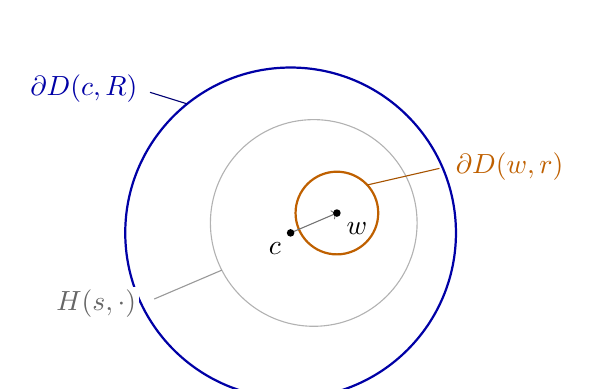
\begin{tikzpicture}[scale=1.05]
 \draw[blue!65!black,thick] (0,0) circle (2);
 \draw[black!30] (.28,.12) circle (1.25);
 \draw[orange!75!black,thick] (.56,.24) circle (.5);
 \draw[->,black!55] (0,0)--(.56,.24);
 \fill (0,0) circle (1.3pt) node[below left] {\(c\)};
 \fill (.56,.24) circle (1.3pt) node[below right] {\(w\)};
 \draw[blue!45!black] (-1.7,1.7)--(-1.25,1.56);
 \node[blue!65!black,fill=white,inner sep=1pt]
    at (-2.5,1.75) {\(\partial D(c,R)\)};
 \draw[orange!65!black] (.93,.58)--(1.8,.78);
 \node[orange!75!black,fill=white,inner sep=1pt]
    at (2.65,.8) {\(\partial D(w,r)\)};
 \draw[black!40] (-1.65,-.8)--(-.83,-.45);
 \node[black!60,fill=white,inner sep=1pt] at (-2.35,-.85) {\(H(s,\cdot)\)};
\end{tikzpicture}
\caption{The explicit family stays inside the outer disc and at distance
at least \(r\) from the pole. The proof samples rational parameters and
uses affine cancellation at the image vertices.}
\label{fig:homotopy}
\end{figure}

Subdivide each of the four parameter squares into \(N^2\) squares and
split each into two oriented triangles. Map their vertices by \(H_j\).
There are \(8N^2\) image triangles, each with
\[
 D_\triangle\le8R/N,\qquad P\le24R/N.
\]
Therefore
\begin{equation}\label{eq:chainconstants}
 \sum PD_\triangle\le1536R^2,\qquad \sum P\le192RN.
\end{equation}
Choose the parameter orientations so that the total boundary is the outer
sampled circle minus the inner sampled circle. Interior edges cancel,
and seams cancel by \(H_j(s,1)=H_{j+1}(s,0)\), cyclically in \(j\).
Every shared node uses the same canonical rational code and precision.

Image triangles may overlap, reverse orientation or degenerate. Only
their algebraic boundaries matter. No Jordan theorem, planar triangulation
theorem or inside/outside decision is required. An analytic collar
around image triangles is unnecessary: the local estimate uses only
vertices, which are certified by \eqref{eq:homoin}--\eqref{eq:homosep}.

\subsection{The finite Cauchy estimate}\label{sec:cfinite}

If \(8R/N\le2^{-\mu_g(k)}\), summing \eqref{eq:triangle} gives the rational
inequality
\begin{equation}\label{eq:gridestimate}
 \norm{T_{N,p}^{\rm out}(g)-T_{N,p}^{\rm in}(g)}
 \le1536R^2\,2^{-k}+(384RN+1536R^2)2^{-p}.
\end{equation}
Each endpoint circle has four pieces with Lipschitz constant at most
\(4R\). Its quadrature error from \eqref{eq:contourerror} is at most
\(64KR^2/N+16R2^{-p}\). Hence
\begin{align}
 \norm{\Int_{\rm out}(g)-\Int_{\rm in}(g)}
 \le1536R^2\,2^{-k}
      +\frac{128KR^2}{N}
      +(384RN+1536R^2+32R)2^{-p}.\label{eq:homofinite}
\end{align}
The proof used the finite grid estimate, followed by two explicit
quadrature comparisons, never an induction on equality of real integrals.

On the inner circle,
\[
 \norm{\frac{f(z)-f(w)}{z-w}}
 \le L\norm{z-w}\norm{(z-w)^{-1}}\le2L.
\]
Its taxicab variation is at most \(16r\). The computed kernel moment gives
\begin{equation}\label{eq:smallcircle}
 \norm{\Int_{\rm in}(g)-2\pi i f(w)}\le32Lr.
\end{equation}
These inequalities first hold for finite sums with their sample errors,
and then for names by the quadrature estimates.

\subsection{The explicit precision schedule}\label{sec:cschedule}

For a raw residual \(2^{-q}\), take
\begin{align}
 r&=\min\left(\delta,\frac{2^{-q}}{128(L+1)}\right),&
 U&=2/r,&K&=LU+MU^2,\label{eq:cs1}\\
 C_g&=\max(1,U,BU^2+MU^3),&
 s&=\sigma(C_g),&
 \mu_g(k)&=\max\{\mu(k+s+1),k+s+1\},\notag\\
 k&=q+\sigma(1536R^2)+2,\notag\\
 m&=\max\{\mu_g(k)+\sigma(8R),\
                        q+\sigma(512KR^2)\},&
 N&=2^m,\label{eq:cs2}\\
 p&=q+\sigma(384RN+1536R^2+32R)+2.\label{eq:cs3}
\end{align}
Every operation is primitive recursive. The mesh condition holds, each
of the three terms of \eqref{eq:homofinite} is at most \(2^{-q}/4\),
and \(32Lr\le2^{-q}/4\). Thus
\begin{equation}\label{eq:crates}
 \norm{\Int_{\partial D(c,R)}\frac{f(z)}{z-w}-2\pi i f(w)}
       \le2^{-q}\qquad\text{for every }q.
\end{equation}
The outer integral's canonical name uses its fixed boundary margin
\(\delta\). The auxiliary radius and meshes vary only with the precision
requested of the proof; they do not change the integral being defined.

To obtain literal rational statements at an output approximation index,
replace each named quantity by its canonical approximation and add the
errors from Section~\ref{sec:data}. Fixing those output indices and
varying \(q\), rational closure gives the cross-index equality of names.
Alternatively, for output tolerance \(2^{-a}\), use \(q=a+3\) and
evaluate the outer integral, \(\pi\) and \(f(w)\) with total error at most
\(2^{-a-2}\); \eqref{eq:producterror} gives the needed shifts.
This proves Theorem~\ref{thm:cpreview}.

\subsection{A named interior point}

Suppose \(w\) is a regular PR complex name with \(|w-c|\le R-\delta\).
Take a rational approximation \(w_e\) with taxicab error
\(e\le\delta/2\). It has certified rational margin \(\delta/2\).
The value \(f(w)\) is the explicit Lipschitz extension of the rational
evaluator, with input-change error at most \(Le\).

On the outer circle the two denominators have Euclidean lower bounds
\(\delta\) and \(\delta/2\), so
\[
 \norm{(z-w)^{-1}-(z-w_e)^{-1}}\le8e/\delta^2.
\]
The total taxicab variation is at most \(16R\), and
\(\norm{(2\pi i)^{-1}}\le1/4\). Therefore
\begin{equation}\label{eq:wextension}
 \norm{\frac1{2\pi i}\Int_\Gamma\frac{f(z)}{z-w}
       -\frac1{2\pi i}\Int_\Gamma\frac{f(z)}{z-w_e}}
       \le32MR e/\delta^2.
\end{equation}
Choosing
\[
 e\le\min\{\delta/2,\
     2^{-q-\sigma(L+32MR/\delta^2)-2}\}
\]
and applying the rational-point formula proves the named-point formula.
It uses a fixed PR name with an explicit margin, not a choice of an
arbitrary real point.

\section{Higher derivatives and the complex Taylor expansion}\label{sec:analytic}

\subsection{A finite inverse-power identity}

For \(m\ge1\), \(u\ne0\), \(u-h\ne0\),
\begin{equation}\label{eq:inversepower}
 (u-h)^{-m}-u^{-m}-mh\,u^{-m-1}
 =h^2\sum_{j=0}^{m-1}(j+1)u^{-j-2}(u-h)^{-(m-j)}.
\end{equation}
Put \(p=u^{-1}\), \(q=(u-h)^{-1}\), so \(q-p=hpq\).
Expand \(q^m-p^m=(q-p)\sum_{\ell<m}q^{m-1-\ell}p^\ell\).
Subtract \(mh p^{m+1}\), use the power-difference identity on the
remaining differences, and collect the finite terms.
This proves \eqref{eq:inversepower}; it also follows after clearing
denominators from \eqref{eq:power2}.

If \(|u|\ge d\), \(|h|\le d/2\), both inverse magnitudes are at most \(2/d\).
Thus
\begin{equation}\label{eq:inversepowerbound}
 |(u-h)^{-m}-u^{-m}-mh\,u^{-m-1}|
 \le C_m(d)|h|^2,\qquad
 C_m(d)=\frac{m(m+1)}2\left(\frac2d\right)^{m+2}.
\end{equation}
This is finite algebra, uniform in \(m\).

\subsection{Construct the derivative tower}

For interior points \(w\) satisfying \(|w-c|\le R-d\), where \(d>0\), define
\begin{equation}\label{eq:Fn}
 F_n(w)=\frac{n!}{2\pi i}\Int_\Gamma
                  \frac{f(z)}{(z-w)^{n+1}},\qquad n\ge0.
\end{equation}
These are jointly PR names. On separated contour points the unnormalized
integrand has taxicab bound \(MU^{n+1}\), \(U=2/d\), and Lipschitz constant
\[
 K_n=LU^{n+1}+M(n+1)U^{n+2}.
\]
This follows by the finite power-difference identity. The contour name
and the factorial and reciprocal precision shifts are consequently PR.
When comparing \(w\) and \(w+h\) with \(|h|\le d/2\), use the shared
lower bound \(d/2\) in their approximation routines. Valid changes of
these bounds do not change the contour value.

Cauchy's formula says \(F_0=f\). Apply \eqref{eq:inversepowerbound} with
\(m=n+1\), multiply by \(f(z)\), and integrate. The circle has Euclidean
length \(2\pi R\), so
\begin{equation}\label{eq:Fderivative}
 |F_n(w+h)-F_n(w)-hF_{n+1}(w)|
 \le n!MR C_{n+1}(d)|h|^2\qquad(|h|\le d/2).
\end{equation}
Thus \(F_n'=F_{n+1}\) with an explicit uniform remainder modulus on every
smaller disc. A taxicab derivative modulus is
\[
 \max\{\sigma(2/d),\, k+1+\sigma(n!MR C_{n+1}(d))\}.
\]
Indeed, \(\norm v\le2|v|\) and \(|h|\le\norm h\); the extra precision
step absorbs the factor two. The first threshold ensures \(|h|\le d/2\).

This constructs the higher derivatives and proves \eqref{eq:derivintro}.
Uniqueness agrees with any already supplied derivative coefficient:
compare two certificates at a sufficiently small positive rational real
increment, divide by that increment and make both errors arbitrarily
small. The increment is explicitly bounded by the interior margin.
Rational closure proves equality. There is no intermediate-point choice.

At the center the length estimate gives the usual Cauchy bound
\begin{equation}\label{eq:cauchybound}
 |f^{(n)}(c)|\le n!M/R^n.
\end{equation}
At boundary distance \(d\), the corresponding bound is \(n!MR/d^{n+1}\).
The Euclidean integral bound used here follows for finite rational sums
by the triangle inequality and then for names. The speed of the rational
circle is itself a rational function, so the length calculation uses no
additional existence theorem for integrals.

\subsection{Finite expansion and convergence rate}

For \(N\ge1\), \(u\ne0\), \(u-x\ne0\), finite geometric algebra gives
\begin{equation}\label{eq:geometrickernel}
 \frac1{u-x}=\sum_{j=0}^{N-1}\frac{x^j}{u^{j+1}}
                        +\frac{x^N}{u^N(u-x)}.
\end{equation}
Apply Cauchy's formula at \(c+x\), put \(u=z-c\), and integrate this
\emph{finite} identity. It yields
\[
 f(c+x)=\sum_{j<N}\frac{f^{(j)}(c)}{j!}x^j+E_N(x).
\]
If \(|x|\le\theta R\), \(0\le\theta<1\), then
\(|u|=R\), \(|u-x|\ge(1-\theta)R\).
The contour length \(2\pi R\) and normalization \(1/(2\pi)\) give
\begin{equation}\label{eq:analytictail}
 |E_N(x)|\le C\theta^N,\qquad C=M/(1-\theta).
\end{equation}
This proves \eqref{eq:ctailintro} without termwise differentiation of an
infinite series.

A primitive recursive cutoff is
\[
 \varepsilon=1-\theta,\quad
 m=\lceil1/\varepsilon\rceil,\quad
 N=m\bigl(q+\sigma(C)+1\bigr).
\]
Quantifier-free induction proves
\((1-\varepsilon)^j(1+j\varepsilon)\le1\): its step uses
\[
 (1-\varepsilon)(1+(j+1)\varepsilon)
       =1+j\varepsilon-(j+1)\varepsilon^2\le1+j\varepsilon.
\]
Hence \(\theta^m\le1/2\) and \(C\theta^N\le2^{-q-1}\).
The case \(\theta=0\) is included. The complex Taylor series therefore has
an explicit PR convergence modulus on every supplied smaller disc.

\section{Why the proofs fit quantifier-free induction}\label{sec:ipra}

\subsection{The arithmetic statements}

For Taylor the principal object-theory statement is \eqref{eq:tfinite},
with rational arithmetic and finite sums replaced by their natural-number
codes. Its hypotheses are the finite bound and derivative instances at
\(t_i\), for \(j\le n\), \(i<N\). The universal input contracts imply
these instances by intuitionistic universal elimination.

For Cauchy the principal statement is \eqref{eq:gridestimate}. Its terms
compute the rational homotopy nodes, normalized evaluator inputs,
trapezoidal sums and the numerical error. Its hypotheses are the finite
derivative instances and rational geometry bounds at the vertices.
The explicit schedule supplies the mesh and separation inequalities.

The integral construction, kernel normalization and conversions to name
equality are further first-order derivations. Universal precision
quantifiers are introduced \emph{after} the finite estimates are proved.
The schematic conclusion is
\[
 \ipra\ \vdash\
   \mathcal H(\mathbf a)\longrightarrow
                    \forall q\,\mathcal E(\mathbf a,q),
\]
where \(\mathbf a\) denotes numerical data, \(\mathcal H\) expresses the
coherence, bounds, regularity and separation assumptions for fixed PR
procedures, and \(\mathcal E\) is the requested rational precision claim.
There are no function-sort quantifiers.

\subsection{The induction ledger}

\begin{longtable}{>{\raggedright\arraybackslash}p{.25\textwidth}
                  >{\raggedright\arraybackslash}p{.66\textwidth}}
\toprule
Construction & Quantifier-free invariant\\\midrule
\endhead
Finite arithmetic &
Equality of recursive sums, products or powers; denominator positivity
and numerical index bounds.\\
Refinement &
Equality of repeated weights and the rational bound on the partial
difference of two finite sums.\\
FTC and Taylor &
The partial telescoping identity and accumulated local rational error
bound, with precision and mesh fixed as numerical parameters.\\
Affine triangle &
A ring identity in rational-complex coordinates.\\
Homotopy grid &
The accumulated oriented-edge expression, exact cancellation of matching
sampled edges, and the rational sum of triangle errors.\\
Kernel powers &
The finite inverse-power or geometric identity and a rational bound on its
finite coefficient sum.\\
Geometric tail &
\((1-\varepsilon)^j(1+j\varepsilon)\le1\), expressed by rational
cross multiplication.\\
Finite premises &
A PR Boolean fold equal to \(1\).\\\bottomrule
\end{longtable}

The input assumptions may contain universal quantifiers. They stay in the
side context and are instantiated at the numerical indices needed by each
step. They are not inserted into the induction formula.
Equality of names, which quantifies over all precisions, is never used as
an induction invariant.

This is the logical reason the human proofs have the claimed arithmetic
strength. Computability alone would not suffice: a construction might
need a non-PR search bound, or its proof might use stronger induction.
Here both the computation bounds and the finite induction assertions
are explicit.

\subsection{Constructive principles}

The proofs use no excluded middle for arbitrary formulas, choice or
Markov's principle. Their case distinctions concern integers and
rationals. There is no arbitrary-real compactness argument, an
extremum-attainment theorem, an integral mean-value theorem, or an
unbounded search for a suitable mesh.
The results are schemas for certified PR presentations; they do not assert
that every classical function is an object of first-order arithmetic.

\section{A concrete Lean formalization path}\label{sec:lean}

\subsection{Source-audited APIs and the target}

The inspected namespace is \code{LeanProofs.ConciseIPRA}.
The following declarations exist at the pinned revision:
\begin{center}\small
\begin{tabular}{>{\raggedright\arraybackslash}p{.33\textwidth}
                >{\raggedright\arraybackslash}p{.57\textwidth}}
\toprule
Module & Relevant declarations\\\midrule
\code{PR.lean} &
\code{PR}, \code{PTm}, \code{PRAAx}, \code{PRA.qfInd}\\
\code{Deduction.lean} &
\code{Prf}, substitution, weakening, cut and equality helpers\\
\code{PRAToScalar.lean} &
\code{FromPRA.code}, \code{FromPRA.sigma}, \code{FromPRA.interp}\\
\code{TeqReflect.lean} &
\code{chi}, \code{chi\_iff}, \code{Teq.qfInd}\\
\code{NativeBiInterpretation.lean} &
\code{NFm.ofPRA}, \code{pra\_iff\_native}\\\bottomrule
\end{tabular}
\end{center}
The existing \code{pra\_iff\_native} theorem is precisely the equivalence
between a \code{Prf PRAAx} derivation and an \code{NPrf} derivation after
mapping formulas and the context with \code{NFm.ofPRA}.
The supplied native bridge applies its forward direction:
\begin{lstlisting}
theorem native_of_ipra
    (h : Prf PRAAx Gamma phi) :
    NPrf (Gamma.map NFm.ofPRA) (NFm.ofPRA phi) :=
  pra_iff_native.mp h
\end{lstlisting}
The substantive target is a derivation
\begin{lstlisting}
Prf PRAAx hypotheses finitePrecisionConclusion
\end{lstlisting}
followed by universal closure of the precision parameter.
An ambient Lean theorem about \code{Real}, \code{Complex},
\code{intervalIntegral} or \code{circleIntegral} would be a useful
semantic comparison but would not establish this target.

Mathlib already provides ordinary analytic Taylor and Cauchy results
\cite{mathlibtaylor,mathlibcauchy}. They can validate the interpretation
externally; they do not replace the embedded arithmetic derivations.

\subsection{Implementation layers and precise proof obligations}

\begin{enumerate}[leftmargin=*]
 \item \textbf{Coded arithmetic.}
 Define signed integers, rational pairs, normalization, rational-complex
 operations, comparison, factorial, powers, finite lists and \(\sigma\)
 using \code{PR}. Prove object equations and order lemmas with
 \code{PRA.qfInd}. Canonical rational arguments ensure identical node
 codes on shared edges.

 \item \textbf{Finite algebra.}
 Formalize the power identities, Taylor product split and cancellation,
 affine triangle identity, quotient identity, inverse-power remainder
 and finite geometric identity. The supplied \code{FiniteCore.lean}
 contains semantic algebra scripts for several of these. Replay them
 in the coded object arithmetic: a semantic \code{ring} proof is not
 automatically a \code{Prf PRAAx} proof.

 \item \textbf{Names and integration.}
 Encode the coherence, magnitude, continuity and derivative contracts.
 Implement approximation operations with explicit error shifts.
 Prove the Riemann refinement, finite FTC and contour refinement
 estimates. Each construction returns a PR expression with an arithmetic
 correctness derivation, not an abstract completion object.

 \item \textbf{Taylor.}
 Express \eqref{eq:tfinite} with numerical variables \(n,N,p,r\),
 evaluator terms and finite Boolean premise packets. The inner loop
 proves jet cancellation and the product-error bound; the outer loop
 proves telescoping. Verify \eqref{eq:tschedule}, then the integral
 formula, the polynomial weight integral and the Peano remainder.

 \item \textbf{Cauchy.}
 Encode the rational circle, its derivatives, \(\pi\), the homotopy and
 the grid. Prove the disc/separation predicates, seam identities and
 perimeter/diameter sums. Formalize the oriented-edge fold and
 \eqref{eq:gridestimate}. Add the endpoint quadrature errors and the
 small-circle estimate; verify \eqref{eq:cs1}--\eqref{eq:cs3}.

 \item \textbf{Higher derivatives and analyticity.}
 Prove the inverse-power estimate and construct the joint PR family
 \eqref{eq:Fn}. Its adjacent derivative certificates follow uniformly
 from finite algebra. Prove the Cauchy bounds and the finite geometric
 remainder. The displayed cutoff supplies convergence.

 \item \textbf{Native export and audit.}
 Construct the final formulas in \code{Fm PTm}, close the numerical
 precision universally and apply \code{pra\_iff\_native.mp}.
 Record named \code{\#print axioms} results and source hashes. Check the
 resulting constants against the pinned Lean and Mathlib versions.
\end{enumerate}

\subsection{Delivered formalization work and remaining work}

The actual Lean scripts cover finite telescoping, summation by parts,
finite geometric algebra, the Taylor product split, affine triangle
cancellation, common-edge cancellation and the quotient remainder,
together with the source-level native bridge.
They contain no proof holes or newly postulated analytic axioms.

No Lean executable was available in the producing environment, so these
scripts are explicitly \emph{uncompiled}; successful elaboration and
kernel checking are not claimed. More substantially, the full coded
rational library, finite-precision object derivations and final
Taylor/Cauchy \code{Prf PRAAx} objects remain to be implemented.
The native bridge is the last small step, not a replacement for that work.

The pinned repository specifies Lean \code{v4.32.0} and Mathlib
\code{v4.32.0}. The finite algebra file can be checked in that Mathlib
environment. The native bridge additionally needs the ProveIt module
available through its Lake configuration. The companion roadmap gives
commands and completion gates.

\section{Exact-arithmetic illustrations and reproducibility}\label{sec:validation}

\subsection{Finite algebra and Taylor}

The executable uses Python's standard library, exact \code{Fraction}
arithmetic and a rational-complex pair type. It checks finite identities,
affine triangle cancellation and subdivision, 54 exact polynomial Taylor
instances and their factorial bounds, and a rounded finite Taylor
certificate.

The rounded example uses \(f(t)=1+t+t^2+t^3\), \(n=2\), \(N=64\),
\(p=16\), \(r=4\). It checks the local derivative and magnitude hypotheses
before checking \eqref{eq:tfinite}. The evaluation-error term proportional
to \(N\) is therefore exercised, not merely omitted by using exact data.

\subsection{A certified circle calculation}

For \(f(z)=1+z+z^2\), \(w=1/4+i/8\) and the unit circle, the program
computes exact rational trapezoidal quadrature of the parameter
integrands on four rational pieces. It also computes a rational
approximation \(P_N\) to \(\pi\); the target is \(2P_Nif(w)\).
This is a smooth-parameter quadrature illustration; the main theorem
uses the contour sums and finite homotopy estimate proved above.

The code note derives
\[
 |H_j''(t)|\le87776/125,\qquad |P_N-\pi|\le2/(3N^2).
\]
The exact rational defect is consequently bounded in Euclidean norm by
\[
 \frac{(87776/125)/3+95/48}{N^2}.
\]
Final comparisons use squared Euclidean norms and exact fractions.
\begin{center}
\begin{tabular}{rrr}
\toprule
Samples per quarter & Certified bound & Observed magnitude\\\midrule
64 & \(0.0576290283203125\) & approximately \(7.82\cdot10^{-6}\)\\
128 & \(0.014407257080078125\) & approximately \(1.95\cdot10^{-6}\)\\
\bottomrule
\end{tabular}
\end{center}
Decimals are display-only; exact rational components and comparison
results are stored in the JSON.
These are finite validation examples, not substitutes for the universal
mathematical proof or for a completed Lean/iPRA derivation.

\subsection{Contents and reproduction}

The archive contains:
\begin{itemize}
 \item \code{report.tex} and compiled \code{report.pdf};
 \item Lean algebra scripts, the native bridge and a detailed roadmap;
 \item \code{code/validate\_exact.py}, its explanatory note and
       deterministic \code{validation.json};
 \item provenance, validation records and checksums.
\end{itemize}
From the extracted archive directory:
\begin{lstlisting}
python3 code/validate_exact.py --output code/validation.json
pdflatex -interaction=nonstopmode -halt-on-error report.tex
pdflatex -interaction=nonstopmode -halt-on-error report.tex
\end{lstlisting}
The mathematical argument is standalone; the inspected repository gives
the concrete embedded-theory target for completing the Lean development.

\begin{thebibliography}{99}
\raggedright
\bibitem{prsource}
V. Reshetnikov, ProveIt, \emph{ConciseIPRA/PR.lean}, inspected revision
\code{876ef598f674759da5f084dc34f63ca4e182aae0}.
\url{https://github.com/VladimirReshetnikov/ProveIt/blob/876ef598f674759da5f084dc34f63ca4e182aae0/Logic/PrimitiveRecursiveArithmetic/ConciseIPRA/Lean/ConciseIPRA/PR.lean}.

\bibitem{nativesource}
V. Reshetnikov, ProveIt, \emph{ConciseIPRA/NativeBiInterpretation.lean},
same revision.
\url{https://github.com/VladimirReshetnikov/ProveIt/blob/876ef598f674759da5f084dc34f63ca4e182aae0/Logic/PrimitiveRecursiveArithmetic/ConciseIPRA/Lean/ConciseIPRA/NativeBiInterpretation.lean}.

\bibitem{calculusdraft}
ProveIt draft archive, \emph{calculus\_ipra.zip}, source report and
artifacts inspected at the same revision.
\url{https://github.com/VladimirReshetnikov/ProveIt/blob/876ef598f674759da5f084dc34f63ca4e182aae0/docs/drafts/calculus_ipra.zip}.

\bibitem{cauchydraft}
ProveIt draft archive, \emph{cauchy\_residue\_ipra.zip}, source report and
artifacts inspected at the same revision.
\url{https://github.com/VladimirReshetnikov/ProveIt/blob/876ef598f674759da5f084dc34f63ca4e182aae0/docs/drafts/cauchy_residue_ipra.zip}.

\bibitem{mathlibtaylor}
Mathlib contributors, \emph{Mathlib.Analysis.Calculus.Taylor},
documentation consulted November 15, 2026.
\url{https://leanprover-community.github.io/mathlib4_docs/Mathlib/Analysis/Calculus/Taylor.html}.

\bibitem{mathlibcauchy}
Mathlib contributors, \emph{Mathlib.Analysis.Complex.CauchyIntegral},
documentation consulted November 15, 2026.
\url{https://leanprover-community.github.io/mathlib4_docs/Mathlib/Analysis/Complex/CauchyIntegral.html}.

\bibitem{wikitaylor}
Wikipedia contributors, \emph{Taylor's theorem}, requested reference,
consulted November 15, 2026.
\url{https://en.wikipedia.org/wiki/Taylor%27s_theorem}.

\bibitem{wikicauchy}
Wikipedia contributors, \emph{Cauchy's integral formula}, requested
reference, consulted November 15, 2026.
\url{https://en.wikipedia.org/wiki/Cauchy%27s_integral_formula}.
\end{thebibliography}
\end{document}


